\documentclass{article}

\usepackage{graphicx}
\usepackage{tikz}
\usepackage{tikzsymbols}
\usetikzlibrary{calc,patterns,shapes.geometric}
\pagestyle{empty}
\usepackage[margin=0pt]{geometry}
\geometry{papersize={14in,12in}}

\def\centerarc[#1](#2)(#3:#4:#5){\draw[#1] ($(#2)+({#5*cos(#3)},{#5*sin(#3)})$) arc (#3:#4:#5);}

\begin{document}
	\begin{figure}
		\centering
		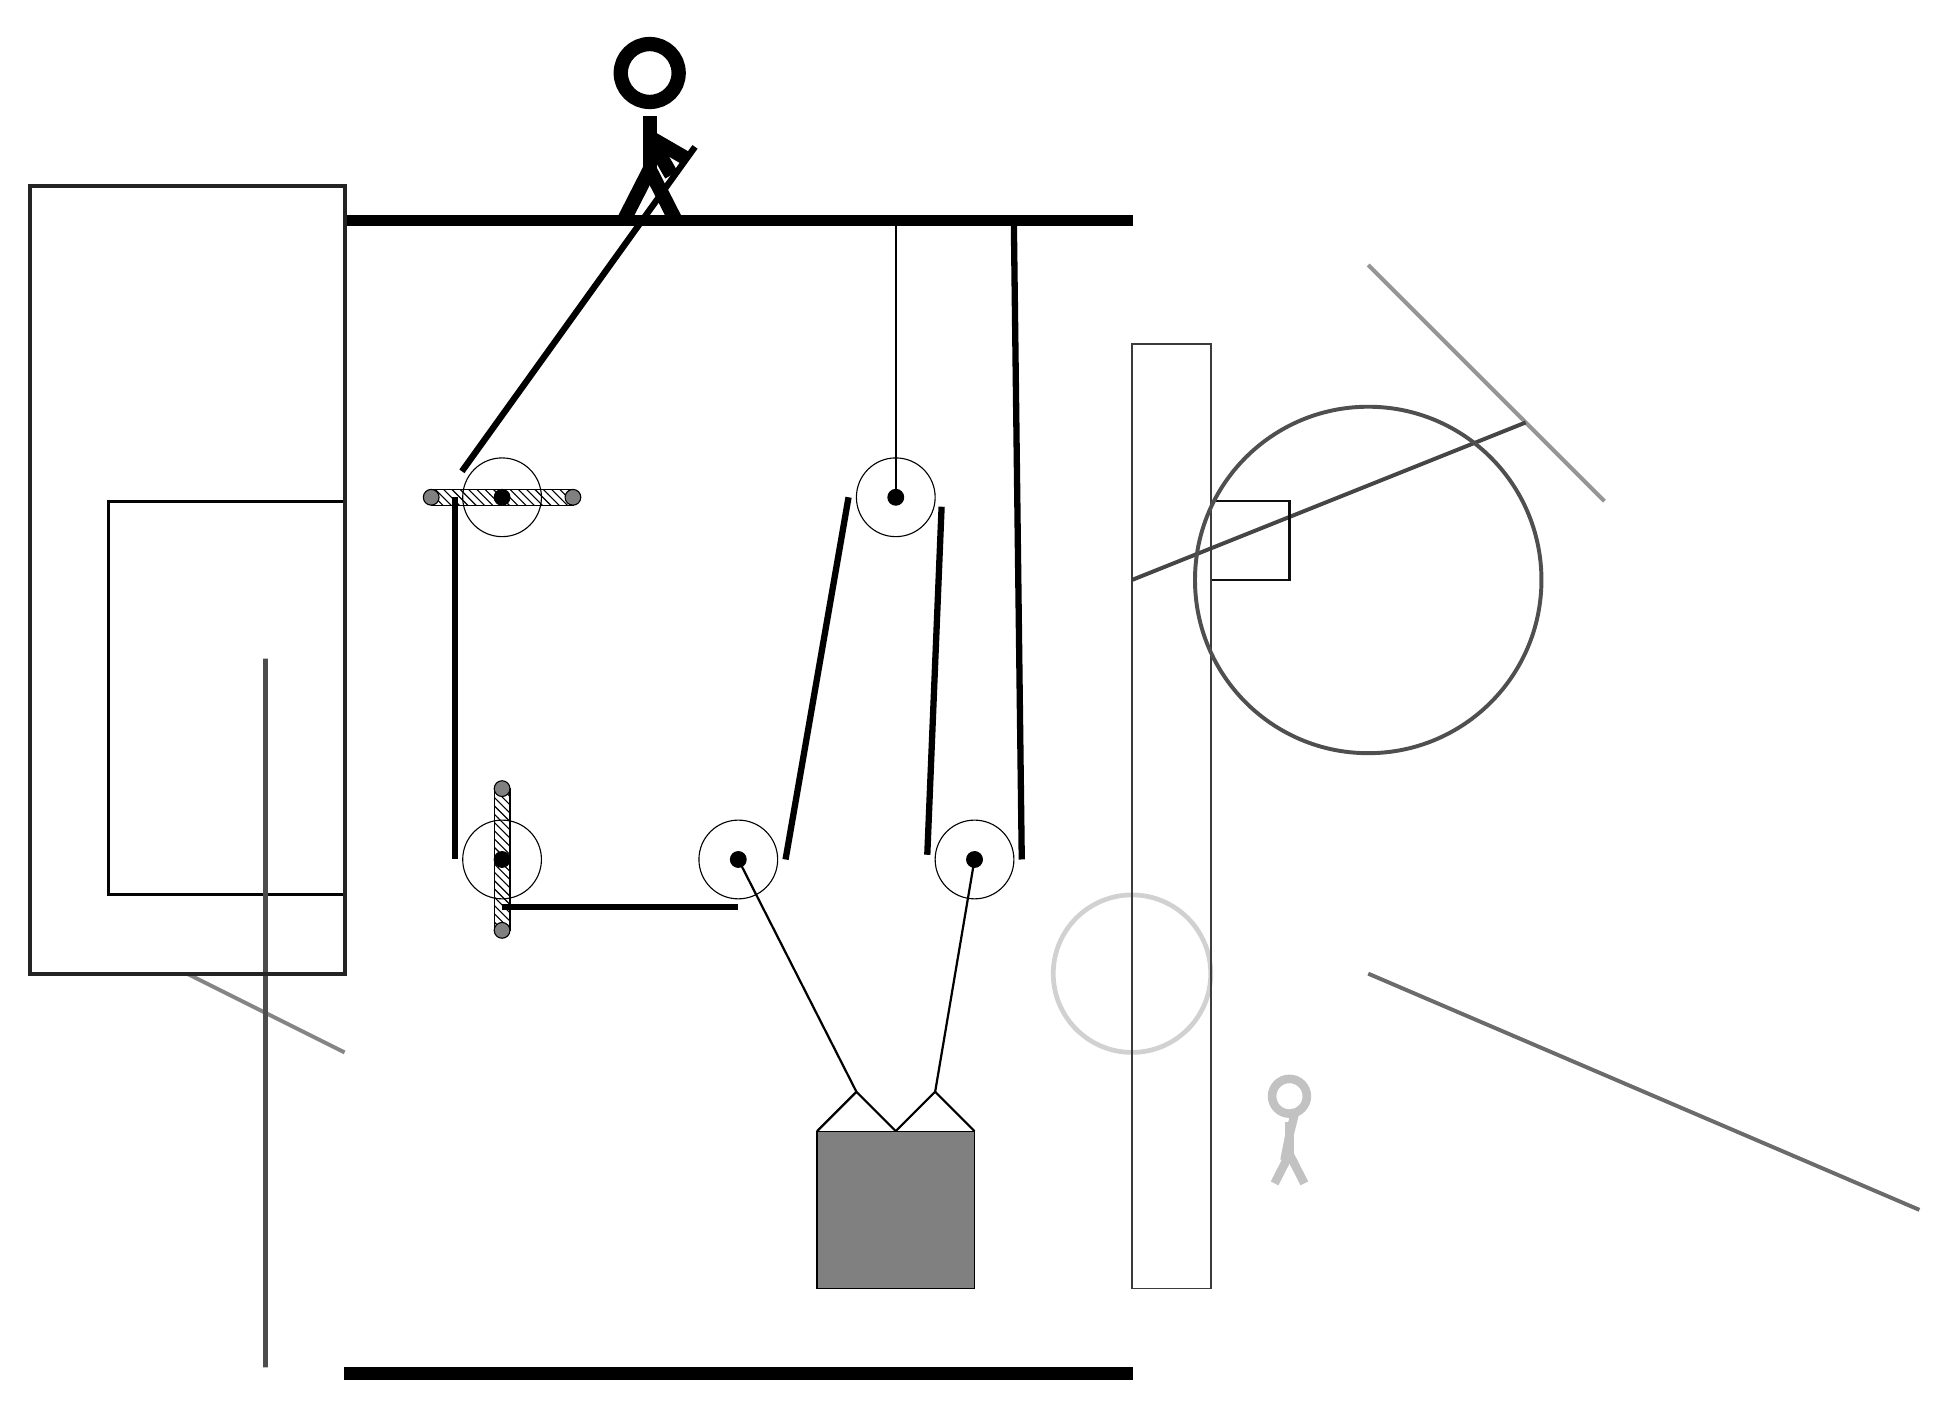
\begin{tikzpicture}
			%%%%% START %%%%%
			
			\draw[fill=black] (-4, 11.5) rectangle (6, 11.625);
			
			\draw (1, 3.45) circle (0.5);
			\draw[fill=black] (1, 3.45) circle (0.1);
			
			\draw (3, 8.05) circle (0.5);
			\draw[fill=black] (3, 8.05) circle (0.1);
			\draw[thick] (3, 8.05) -- (3, 11.5);
			
			\draw (4, 3.45) circle (0.5);
			\draw[fill=black] (4, 3.45) circle (0.1);
			
			\draw[thick] (4, 3.45) -- (3.5, 0.5);
			\draw[thick] (1, 3.45) -- (2.5, 0.5);
			\draw[thick]  (2, 0) -- (2.5, 0.5) -- (3, 0);
			\draw[thick]  (3, 0) -- (3.5, 0.5) -- (4, 0);
			\draw[fill=black!50] (2, 0) rectangle (4, -2);
			
			\draw (-2, 3.45) circle (0.5);
			\draw[fill=black] (-2, 3.45) circle (0.1);
			\draw[pattern=north west lines, pattern color=black] (-2.1, 4.35) rectangle (-1.9, 2.55);
			\draw[fill=black!50] (-2, 4.35) circle (0.1);
			\draw[fill=black!50] (-2, 2.55) circle (0.1);
			
			\draw[line width=0.5mm, color=black!41](9, 11) -- (12, 8);
			
			\draw[line width=0.5mm, color=black!58](9, 2) -- (16, -1);
			\draw[line width=0.4mm, color=black!99] (-4, 3) rectangle (-7, 8);
			\draw[line width=0.5mm, color=black!73](6, 7) -- (11, 9);
			
			\draw[line width=0.3mm, color=black!94] (7, 7) rectangle (8, 8);
			\node[line width=0.3mm, color=black!24] at (8, 0) {\Strichmaxerl[6][79][76]};
			\draw [line width=0.6mm, color=black!18](6, 2) circle (1.0);
			\draw[line width=0.5mm, color=black!48](-4, 1) -- (-6, 2);
			\draw[line width=0.6mm, color=black!70] (-5, 6) rectangle (-5, -3);
			\draw[line width=0.5mm, color=black!86] (-4, 12) rectangle (-8, 2);
			
			\draw[line width=0.2mm, color=black!77] (6, 10) rectangle (7, -2);
			\draw [line width=0.5mm, color=black!69](9, 7) circle (2.2);
			
			\draw (-2, 8.05) circle (0.5);
			\draw[fill=black] (-2, 8.05) circle (0.1);
			\draw[pattern=north west lines, pattern color=black] (-2.9, 8.15) rectangle (-1.1, 7.95);
			\draw[fill=black!50] (-2.9, 8.05) circle (0.1);
			\draw[fill=black!50] (-1.1, 8.05) circle (0.1);
			
			\draw[line width=0.8mm] (0.45, 12.5) -- (-2.51, 8.38);
			\centerarc[line width=0.8mm](-2, 8.05)(135:180:0.6);
			\draw[line width=0.8mm] (-2.6, 8.05) -- (-2.6, 3.45);
			\centerarc[line width=0.8mm](-2, 3.45)(180:270:0.6);
			\draw[line width=0.8mm](-2, 2.85) -- (1, 2.85);
			\centerarc[line width=0.8mm](1, 3.45)(270:360:0.6);
			\draw[line width=0.8mm] (1.6, 3.45) -- (2.4, 8.05);
			\centerarc[line width=0.8mm](3, 8.05)(-20:180:0.6);
			\draw[line width=0.8mm](3.582, 7.93) -- (3.4, 3.51);
			\centerarc[line width=0.8mm](4, 3.45)(160:360:0.6);
			\draw[line width=0.8mm](4.6, 3.45) -- (4.5, 11.5);
			
			\node at (-0.07, 12.7) {\Strichmaxerl[10][120][-30]};
			
			\draw[fill=black] (-4, -3) rectangle (6, -3.15);
			
			%%%%% END %%%%%
		\end{tikzpicture}
	\end{figure}	
\end{document}